\section{Cel Projektu}
Celem projektu jest demonstracja możliwości zrównoleglenia obliczeń Szybkiej Transformaty Fouriera (FFT), na przykładzie przetwarzania obrazów.
\section{Wstęp}
\subsection{Technologia i zakres projektu}
\paragraph{Sposób działania programu}
Działanie programu polega na wczytywaniu obrazów w formacie BMP, poddawaniu ich
transformacji, a następnie zapisywaniu plików wyjściowych. Program dokonuje także transformacji odwrotnej. Możliwe jest zrównoleglenie poprzez uruchomienie kilku procesów (jeden proces na przetwarzanie jednego obrazu wejściowego) oraz skorzystanie z przetwarzania wielowątkowego. Działanie programu przetestowaliśmy na kilkunastu obrazach testowych o rozmiarach od $ 64x64 $ do $ 1024x1024 $.
\paragraph{Technologia i wykorzystane biblioteki}Program został napisany w C\#, do zrównoleglenia wykorzystujemy $ System.Diagnostics $ oraz $ System.Threading $.\\
 Pełna lista bibliotek:\\
 
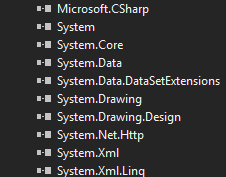
\includegraphics[scale=1]{figures/bibl.png}
\subsection{Wprowadzenie do tematyki FFT}

\paragraph{Zastosowania} Zastosowania transformacji obrazów to m. in.:
\begin{itemize}
	\item Uzyskanie bardziej zwartego (oszczędnego) sposobu kodowania obrazów
	(ich kompresji, np. standard kompresji obrazów JPEG),
	\item Uwidocznienie cech obrazu niezauważalnych w dziedzinie przestrzennej,
	np. zakłóceń okresowych.
\end{itemize}
\subsection{Szczegóły instalacji i uruchomienia programu} 
Aby uruchomić program wystarczy mieć możliwość wykonania pliku $exe$. \\
Przykład uruchomienia:\\

\textit{\Large{FFT.exe filname.bmp filename2.bmp filename3.bmp}}
\section{Opis rozwiązania}
Zrównoleglenie przeprowadziliśmy poprze wprowadzenie wieloprocesowości oraz wielowątkowości.
\paragraph{Wieloprocesowość} Wprowadziliśmy możliwość uruchamiania przetwarzania każdego wczytywanego obrazu z linii poleceń na osobnym procesie.\\
	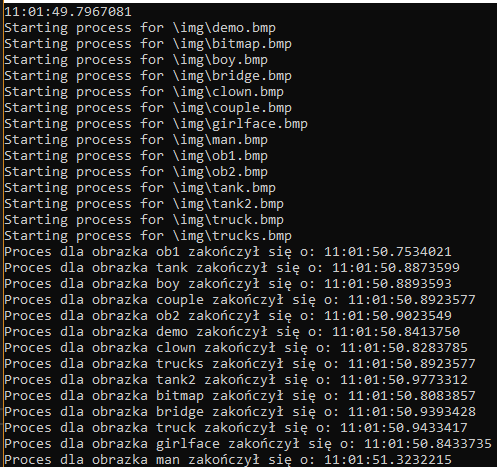
\includegraphics[scale=1]{figures/Par13Wat4.png}
\paragraph{Wielowątkowość} Podczas obliczeń FFT 2D należy wykonać transformatę najpierw na wierszach a następnie na kolumnach. Wykorzystaliśmy to, aby w zależności od ilości wątków definiowanych przez $THREADS$ przydzielać poszczególnym wątkom odpowiednią ilość wierszy, czy kolumn.\\
Należało zadbać o synchroniczny dostęp do tablicy $data$ podczas zapisu wyników częściowych.\\
\begin{lstlisting}
/**
* Moment of synchronization - lock for data table.
**/
 for (int j = 0; j < cols; j++)
	{
	lock(data)
		{
		 data[i, j] = row[j];
		}
	}
\end{lstlisting}
 
\section{Uzyskane rezultaty}
\section{Wnioski}
\begin{itemize}
	\item Po zastosowaniu transformaty w obie strony na obrazku zauważalny jest drobny spadek jakości obrazu.
	\item Zrównoleglenie na procesy poszeczególnych grafik dało bardzo dobre rezultaty i zdecydowanie przyśpieszyło działanie programu przy większej ilości obrazków.
	\item Wersja sekwencyjna jest równie szybka a czasami szybsza dla 2 lub 3 obrazków, ale od 4 i więcej zauważalna jest tendencja przyrostowa czasu wykonywania transformaty. W przeciwieństwie do zrównoleglonej wersji, gdzie czas utrzymuje się mniej więcej na tym samym poziomie.
	\item Użycie zbyt dużej ilości wątków wbrew pozorom daje gorsze rezultaty niż ich mniejsza ilość, np. 8 czy 4. Jest to spowodowane, że program traci czas na uruchomienie poszczególnych wątków, a one same w sobie nie mają dużego obciążenia obliczeniowego
\end{itemize}

